\section{Video Face Clustering}
\label{sec:video_face_clustering}

\begin{figure*}[!ht]
    \centering
    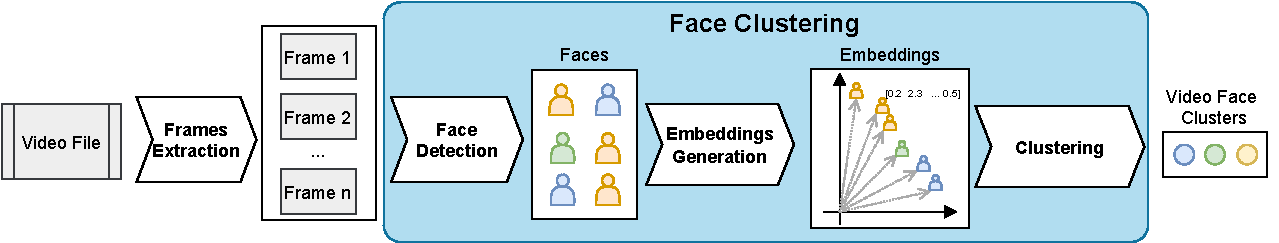
\includegraphics[width=\textwidth]{img/video_face_clustering.pdf}
    \caption{Video face clustering process.}
    \label{fig:video_face_clustering}
\end{figure*}

The core of this dissertation is a method that we call \emph{Video Face Clustering}.
%%
It consists in detecting and grouping faces from different video frames~(ideally from the same actors) extracted from a video file.
%%
Figure \ref{fig:video_face_clustering} depicts this process.
%%
Each of its steps are described in the next paragraphs.


First, we perform \textit{Frames Extraction} by receiving a video file as input and extracting its frames according to a given frame rate. 

The \textit{Face Detection} step uses an object detection model for detecting faces in each of its images.
%%
This model is responsible for returning the bounding boxes of the faces present in the image, specified by the $x$ and $y$ axes coordinates of the upper-left corner and of the lower-right corner of the rectangle that establishes the visual limits that encapsulate each face. 
%%
With these bounding boxes, we can isolate and extract the bounded images, obtaining a dataset composed of images of faces only.

The \textit{Face Detection} step uses an object detection model for detecting faces in each of its images.
%%
This model is responsible for returning the bounding boxes of the faces present in the image, specified by the $x$ and $y$ axes coordinates of the upper-left corner and of the lower-right corner of the rectangle that establishes the visual limits that encapsulate each face. 
%%
With these bounding boxes, we can isolate and extract the bounded images, obtaining a dataset composed of images of faces only.


The objective of the \textit{Embeddings Generation} step is to represent each face image as a vector space in $\mathbb{R}^{n}$.
%%
To achieve that, it processes each of the faces generated in the previous step through a CNN, generating embeddings. 
%%
An embedding is a representation of the input in a lower dimensional space.

In the \textit{Clustering} step, we group embeddings and, consequently, faces that are close in the embedding space using a clustering algorithm. 
%%
The clustering process should produce a partition of the dataset, i.e., each generated cluster represents a specific person, and the union of all clusters covers the whole dataset.

By the end of this process, we expect to have the spatiotemporal localization of the actors present in a video file.
%%
Figure \ref{fig:timeline} shows an example of the results achieved by this method. It contains a timeline of a video with lines coloring the segments that each actor appears.

\begin{figure}[!ht]
    \centering
    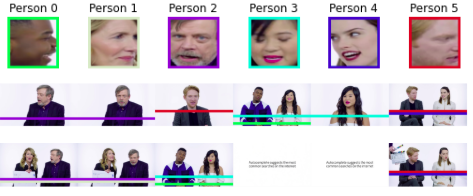
\includegraphics[width=0.6\linewidth]{img/webmedia/timeline2.png}
    \caption{Timeline with tagged frames by their clusters}
    \label{fig:timeline}
\end{figure}

We have evaluated this process by the quality of the clusters generated with different combinations of Convolutional Neural Networks (CNNs) and clustering algorithms. Details about this evaluation will be presented in our dissertation. 

